Una vez elegidos los valores representativos para la generación de lotes de planillas, se realizaron 3 lotes Random de listas de planillas (véase \texttt{rand\_200\_2000\_50.in}, \texttt{rand2\_200\_2000\_50.in}, \texttt{rand3\_200\_2000\_50.in} ) y se calcularon los tiempos de ejecución del algoritmo, obteniendo los resultados en los respectivos .out y las tablas de tiempos en los .times, con las que se obtuvieron los siguientes gráficos.
\newline
\newline
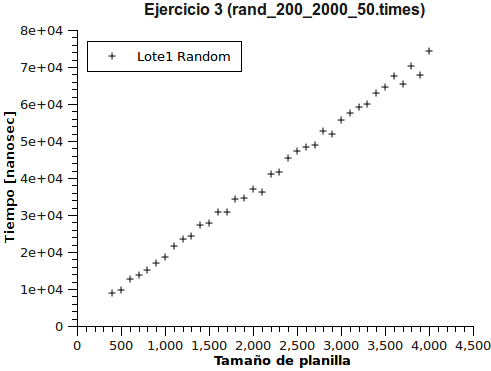
\includegraphics[scale=0.8]{img/ej3/Graph1.png}
\newline
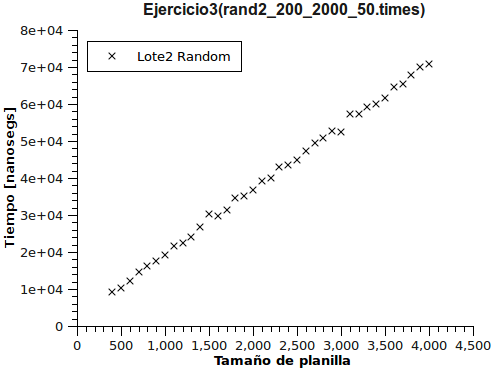
\includegraphics[scale=0.8]{img/ej3/Graph2.png}
\newline
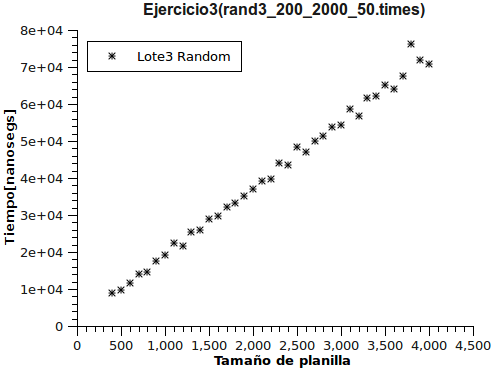
\includegraphics[scale=0.8]{img/ej3/Graph3.png}
\newline


Por otro lado se realizó un lote Worst o Peor caso,(véase \texttt{worst\_200\_2000\_50.in}) y se obtuvo el siguiente gráfico de la tabla de tiempos .

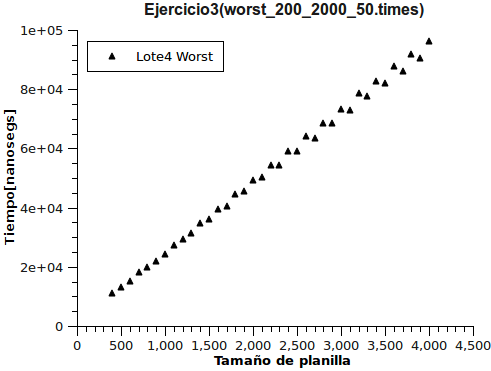
\includegraphics[scale=0.8]{img/ej3/Graph4.png}

